\section{Introducción}

\subsection{Generalidades sobre la clasificación de los virus}

Desde un enfoque evolutivo, un organismo puede ser definido como la unidad 
elemental de un linaje [genético] continuo y con una historia evolutiva 
individual (\cite{luria_general_1978}). Los virus son organismos acelulares 
con genomas constituidos por ácidos nucleicos, que se replican obligadamente 
dentro de células hospedadoras utilizando los ribosomas y la maquinaria 
metabólica del huésped, sintetizando un conjunto de componentes que se 
autoensamblan formando viriones; partículas infectivas que protegen al 
genoma viral y permiten su transferencia a otras células 
(\cite{claverie_giant_2016,koonin_viruses_2021,nasir_investigating_2020,
rybicki_chapter_2023}).

En las últimas dos décadas, ha habido un avance significativo en la 
clasificación de los virus. Anteriormente, se utilizaba una taxonomía basada 
en características fenotípicas, como la estructura del virión, el rango de 
hospedación y la epidemiología. Sin embargo, actualmente la clasificación 
de los virus se ha transformado, adoptando una aproximación similar a la de 
los organismos celulares. Esta nueva clasificación se fundamenta 
principalmente en datos genómicos y filogenéticos, permitiendo conocer y 
reflejar sus relaciones evolutivas 
(\cite{koonin_origins_2015,koonin_global_2020,simmonds_virus_2017})

Los principios, procedimientos y nomenclatura empleados para nombrar y 
clasificar a los organismos, incluyendo los virus, están sujetos a la 
regulación de comités científicos internacionales. El \textit{International 
Committee on Taxonomy of Viruses} (ICTV) es responsable de la taxonomía 
viral, de manera similar a cómo el \textit{International Committee on 
Systematics of Prokaryotes} (ICSP) se encarga de la denominación de especies 
de bacterias y arqueas, o la \textit{International Commission on Zoological 
Nomenclature} (ICZN) se encarga de las animales 
(\cite{iczn_about_nodate,lefkowitz_virus_2018,oren_international_2023})

La aparición y estandarización de la nomenclatura binomial es un hecho 
bastante reciente en virología. Los nombres de los virus previos a la 
ratificación de la norma en 2021 han pasado a ser nombres comunes, siendo en
la actualidad asunto del ICTV la designación de los nombres científicos de 
todas las especies reconocidas (\cite{zerbini_differentiating_2022}). 
A modo de ejemplo: el virus del salmón del Pacífico (PsNV) pertenece al 
género \textit{Alphapironavirus} y a la especie \textit{Alphapironavirus 
bona}.

Aunque la nomenclatura binomial se ha convertido en el formato oficial para 
nombrar a las especies, muchas de las definidas antes de la aprobación de 
esta regla aún no cumplen con este formato. Esta particularidad transitoria 
también afecta de forma significativa a las especies de la familia 
\textit{Coronaviridae}. Por ello, en este trabajo se dará preferencia al uso
de los nombres comunes, los cuales siguen siendo populares y ampliamente 
utilizados en la literatura científica.

\subsection{Taxonomía de los coronavirus}

Dentro del orden \textit{Nidovirales}, los miembros de la familia 
\textit{Coronaviridae} se distribuyen en varias subfamilias que infectan a 
diversos grupos de vertebrados. Según el último reporte del ICTV sobre la 
taxonomía de estos virus, los tradicionalmente conocidos como coronavirus, 
que afectan a aves y mamíferos, se agrupan dentro de la subfamilia 
\textit{Orthocoronavirinae} (\cite{woo_family_2023}). Los estudios 
metagenómicos han ampliado el conocimiento sobre el rango de hospedación de 
esta familia, añadiendo dos nuevas subfamilias: \textit{Letovirinae} 
(\cite{bukhari_description_2018}) (Bukhari et al., 2018), que afectan a 
anfibios, y \textit{Pitovirinae}, presente en peces óseos 
(\cite{mordecai_endangered_2019}). Además, se ha reconocido la existencia de
secuencias de coronavirus encontradas en reptiles 
(\cite{shi_evolutionary_2018}) y peces agnatos (\cite{miller_slippery_2021}), 
las cuales están pendientes de revisión formal.

Hasta la fecha de realización de este trabajo, se ha reconocido una única 
especie para las subfamilias \textit{Letovirinae} y \textit{Pitovirinae}. 
La mayoría de los coronavirus conocidos pertenecen a la subfamilia 
\textit{Orthocoronavirinae} y se distribuyen en cuatro géneros: 
\textit{Alphacoronavirus}, \textit{Betacoronavirus}, 
\textit{Gammacoronavirus} y \textit{Deltacoronavirus} 
(\cite{woo_family_2023}).

Los coronavirus humanos que causan resfriados comunes (HCoVs) se clasifican 
en los géneros \textit{Alphacoronavirus} y \textit{Betacoronavirus}. En el 
género \textit{Alphacoronavirus} se encuentran el HCoV-NL63 y el HCoV-229E, 
mientras que en el género \textit{Betacoronavirus} se incluyen el HCoV-HKU1 
y el HCoV-OC43 (\cite{liu_human_2021}). Además, dentro del género 
\textit{Betacoronavirus}, existen otros coronavirus zoonóticos pandémicos 
capaces de causar enfermedades graves, como el síndrome respiratorio agudo 
severo (SARS), causado por los virus SARS-CoV y SARS-CoV-2, y el síndrome 
respiratorio de Oriente Medio (MERS), causado por el MERS-CoV 
(\cite{peiris_severe_2021}). Es importante destacar que, a pesar de sus 
diferencias clínicas significativas, los virus del SARS se clasifican 
taxonómicamente dentro de la especie \textit{Severe acute respiratory 
syndrome-related coronavirus} (\cite{gorbalenya_species_2020}).

Hasta el año 2021, los reportes de las infecciones humanas por coronavirus 
se limitaban a especies de alfa- y betacoronavirus; hasta la identificación 
de secuencias del deltacoronavirus porcino (PoCoV-HKU15) en muestras de 
sangre de tres niños haitianos con un cuadro febril agudo inespecífico 
(\cite{lednicky_independent_2021}). Un año más tarde se reportó en Malasia 
el salto de virus de la gastroenteritis transmisible (TGEV) caninos a 8 
pacientes ingresados por neumonía durante 2017--2018 
(\cite{vlasova_novel_2022}). Estos hallazgos, dos años después de la 
pandemia mundial causada por el SARS-CoV-2, resaltan nuevamente la 
posibilidad de que nuevos coronavirus, previamente no asociados a los 
humanos, puedan realizar saltos zoonóticos que vuelvan a poner en riesgo 
nuestra salud (\textbf{Figura 1}).

\newpage

\begin{figure}[!ht]
    \centering
    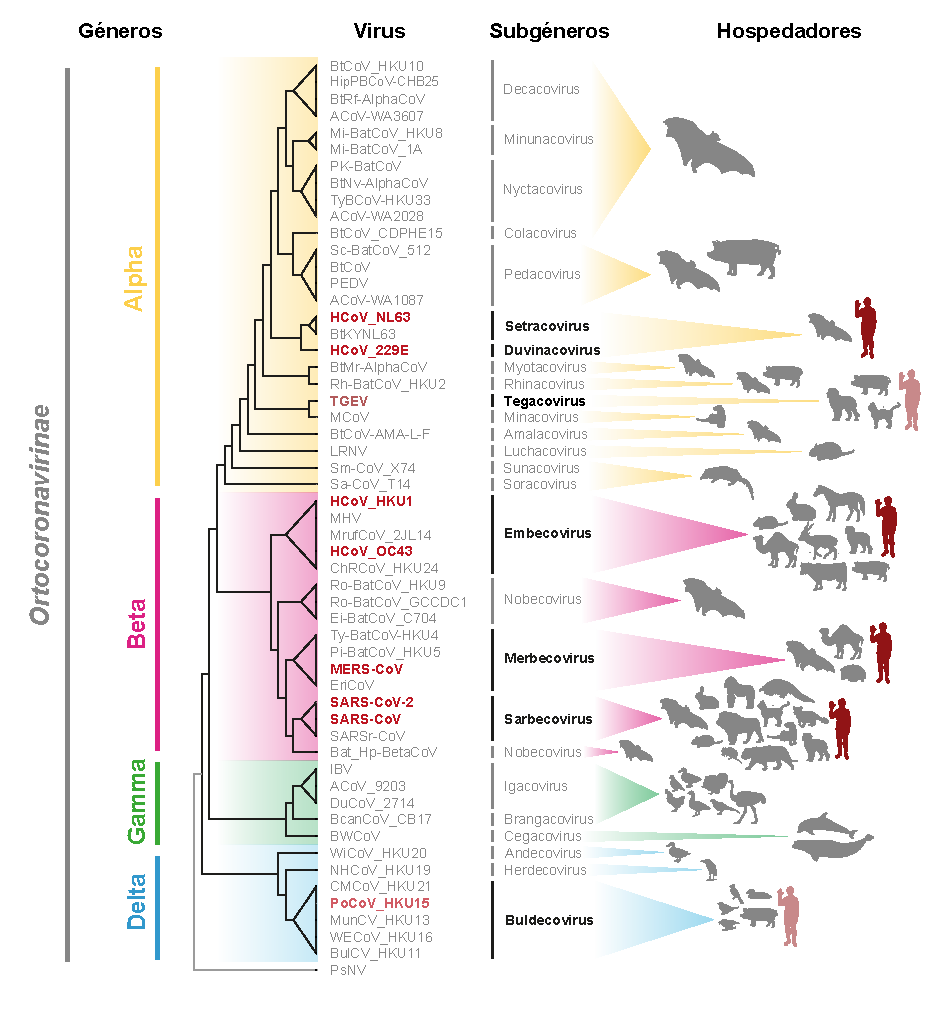
\includegraphics[width=1\textwidth]{img/fig1.pdf}
    \caption{Cladograma de la subfamilia Orthocoronavirinae enraizado a 
    partir de la secuencia del PsNV (subfamilia \textit{Pitovirinae}), con sus 
    relativos hospedadores agrupados por subgéneros según el último informe 
    del ICTV (\cite{woo_family_2023}). En términos generales, los virus de 
    los géneros \textit{Alphacoronavirus} y \textit{Betacoronavirus} se han 
    detectado en una amplia gama de mamíferos, mientras que los géneros 
    \textit{Deltacoronavirus} y \textit{Gammacoronavirus} se han encontrado 
    principalmente en aves. Los hospedadores se indican a través de siluetas 
    tomadas de PhyloPic (\cite{keesey_phylopic_2023}). Los virus que 
    infectan a los seres humanos se marcan en un color rojo intenso, 
    mientras que aquellos cuyo reporte ha sido ocasional se resaltan en un 
    tono más suave. Los nombres completos de los virus y sus especies 
    asociadas quedan recogidos en la (\textbf{Tabla A1}), disponible en 
    anexos. La figura es de elaboración propia para este trabajo.}\label{fig:cladogram}
\end{figure}

\subsection{Estructura y genoma de los coronavirus}

En líneas generales, los viriones de la familia \textit{Coronaviridae} son 
partículas esféricas con un diámetro aproximado de 80--160 nm. Presentan una 
envoltura constituida por una bicapa lipídica sobre la que se anclan 
proteínas estructurales de membrana (M), envoltura (E) y espiga (S) 
(\textbf{Figura 2A}). Las proteínas M y E comparten papel en la morfogénesis
del virión, siendo esta última también un factor de virulencia para algunas 
especies (\cite{jimenez-guardeno_pdz-binding_2014,neuman_structural_2011,ye_role_2007}). 
Por otro lado, la proteína S media en el proceso de reconocimiento, 
fijación y entrada a la célula hospedadora (\cite{bosch_coronavirus_2003}). 
Dentro del virión se encuentra la nucleocápside, la cual a su vez está 
constituida por un genoma viral de ARN monocatenario (ARNmc) positivo de 
unas 30 kilobases (Kb) encapsidado por nucleoproteínas (N) que participan en
su síntesis y traducción (\cite{enjuanes_biochemical_2006}) 
(\textbf{Figura 2B}).

\begin{figure}[!ht]
    \centering
    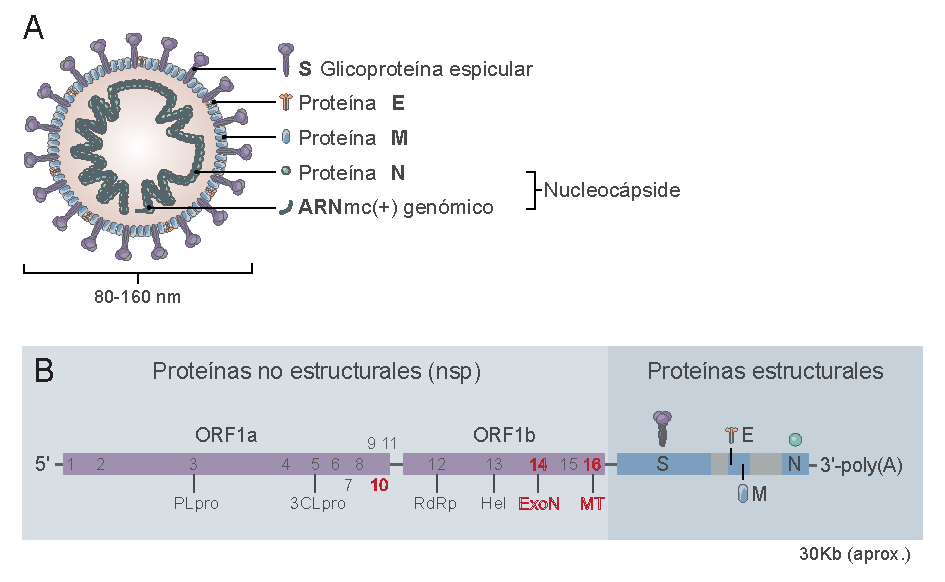
\includegraphics[width=1\textwidth]{img/fig2.pdf}
    \caption{Estructura (\textbf{A}) y genoma (\textbf{B}) de Coronaviridae. 
    El material genético de los coronavirus posee un primer marco abierto 
    de lectura (ORF1a) que codifica proteínas relacionadas con la evasión 
    inmunitaria, mientras el segundo (ORF1b) contiene a la ARN polimerasa 
    viral dependiente de ARN (RdRp) y otras proteínas no estructurales 
    asociadas con la replicación. Ambos ORFs codifican poliproteínas que 
    procesadas por las proteinasas virales (nsp3 y nsp5) dan lugar a cada 
    nsp individual. El otro tercio del genoma contiene los ORFs de las 
    proteínas estructurales del virión. En color rojo se destacan en la 
    figura las actividades enzimáticas clave para este trabajo: exonucleasa 
    (ExoN) y metiltransferasa (MT) desarrolladas por nsp14 y nsp16 
    respectivamente, y nsp10 (cofactor de ambas). Figura tomada y modificada 
    de (\cite{asensio_estructura_2020}).}\label{fig:genome_structure}
\end{figure}

El tamaño de los genomas de la mayoría de los virus de ARN varía dentro de 
un estrecho rango de aproximadamente 1--15 Kb. Esto se considera consecuencia
de la baja fidelidad en sus procesos de replicación, debido a la falta de 
actividad correctora de errores (\Cite{duffy_why_2018,peck_complexities_2018,sanjuan_viral_2010}). 
Los coronavirus sobrepasan ampliamente este límite con sus $\sim$30 kb, 
siendo de los genomas virales de ARN más grandes conocidos. La expansión de 
sus genomas, así como en otras especies del orden Nidovirales, viene 
justificada por la aparición de la capacidad de corrección de errores 
3$'$→5$'$ exoribonucleasa (ExoN) en sus complejos de replicación y 
transcripción (RTC). Dicha actividad enzimática fue descubierta en virus de 
ARN por primera vez en 2003, gracias al análisis bioinformático del genoma 
de SARS-CoV. La identidad de secuencia de exonucleasas celulares compartida 
con un fragmento de la nsp14 de aquel coronavirus evidenciaron la 
funcionalidad de esta última (\cite{snijder_unique_2003}). Tres años más 
tarde, esta predicción fue confirmada in vitro (\cite{minskaia_discovery_2006}).

\subsection{Bases de una posible terapia antiviral pancoronavírica}

Los virus de ARN operan con tasas de error cercanas a los límites 
compatibles con el mantenimiento de su información genética. Existe una 
estrategia antiviral conocida como mutagénesis letal, que implica la 
administración de análogos de nucleósidos, con el objetivo de aumentar las 
tasas de mutación viral y así reducir y eliminar la carga viral 
(\cite{diaz-martinez_lethal_2018,swanstrom_lethal_2022}). 
Algunos ejemplos de la efectividad clínica de estas terapias contra 
enfermedades humanas causadas por virus de ARN son el uso de ribavirina 
contra el dengue y la hepatitis C, o el remdesivir contra el ébola 
(\cite{huggins_prospective_1991,mulangu_randomized_2019,ortega-prieto_extinction_2013}). 
Sin embargo, los intentos de aplicar estos y otros análogos de nucleósidos 
para mitigar la pandemia coronavírica del 2019 (COVID-19) causada por el 
SARS-CoV-2 fracasaron, principalmente por la actividad ExoN de la nsp14 
(\cite{stevaert_nucleoside_2022}).

La nsp14 de los coronavirus es una proteína bifuncional, constituida por el 
dominio aminoterminal con actividad ExoN (nsp14-ExoN) y otro con actividad 
Guanina-N7-metiltransferasa (nsp14-MT) en su extremo carboxilo
(\cite{chen_functional_2009}). Para la estabilización y correcto 
funcionamiento de su sitio activo, la nsp14-ExoN requiere interactuar con 
una unidad de nsp10, mientras que la nsp14-MT lleva a cabo su actividad sin 
la necesidad de un cofactor proteico adicional (\cite{ferron_structural_2018}).

Además, la nsp10 también actúa como cofactor para la actividad de la nsp16. 
Esta última es una enzima con actividad 2'-O-metiltransferasa que, junto con
la actividad de la nsp14-MT, desempeña un papel crucial en la formación de 
la caperuza 5' del genoma viral; estructura protectora que evita el 
reconocimiento del genoma viral por parte del sistema inmunitario innato 
(\cite{pan_n7-methylation_2022}).

Las enzimas eucariotas que realizan actividades semejantes a las de la 
nsp14-ExoN y la nsp16 de los coronavirus presentan estructuras 
considerablemente diferentes y no requieren de cofactores proteicos para 
desempeñar sus funciones (\cite{galloway_mrna_2019,rona_nsp14nsp10_2022}).
Estas diferencias estructurales abren la posibilidad de aprovechar las 
interacciones con la nsp10 como diana antiviral pancoronavírica.

Desde 2020, el equipo de investigación liderado por la Dra. Ana Grande en el
campo de $``$Evolución de virus y terapias antivirales$''$ está trabajando en 
el diseño de posibles pseudoligandos, basados en estructuras del SARS-CoV-2, 
que compitan con los dominios de unión para nsp10 de la nsp14-ExoN y la 
nsp16. Además, se pretende aumentar la efectividad de dicha terapia mediante
su uso combinado con análogos de bases, que dirijan a los coronavirus más 
rápidamente hacia la catástrofe de error por mutagénesis letal 
(\textbf{Figura 3}). Los estudios en relación a este proyecto se llevan a 
cabo en la Universidad de Málaga, en colaboración con el Centro de Biología 
Molecular `Severo Ochoa' y la Universidad de Elche (\cite{grande-perez_nueva_2021}).

\begin{sidewaysfigure}
    \centering
    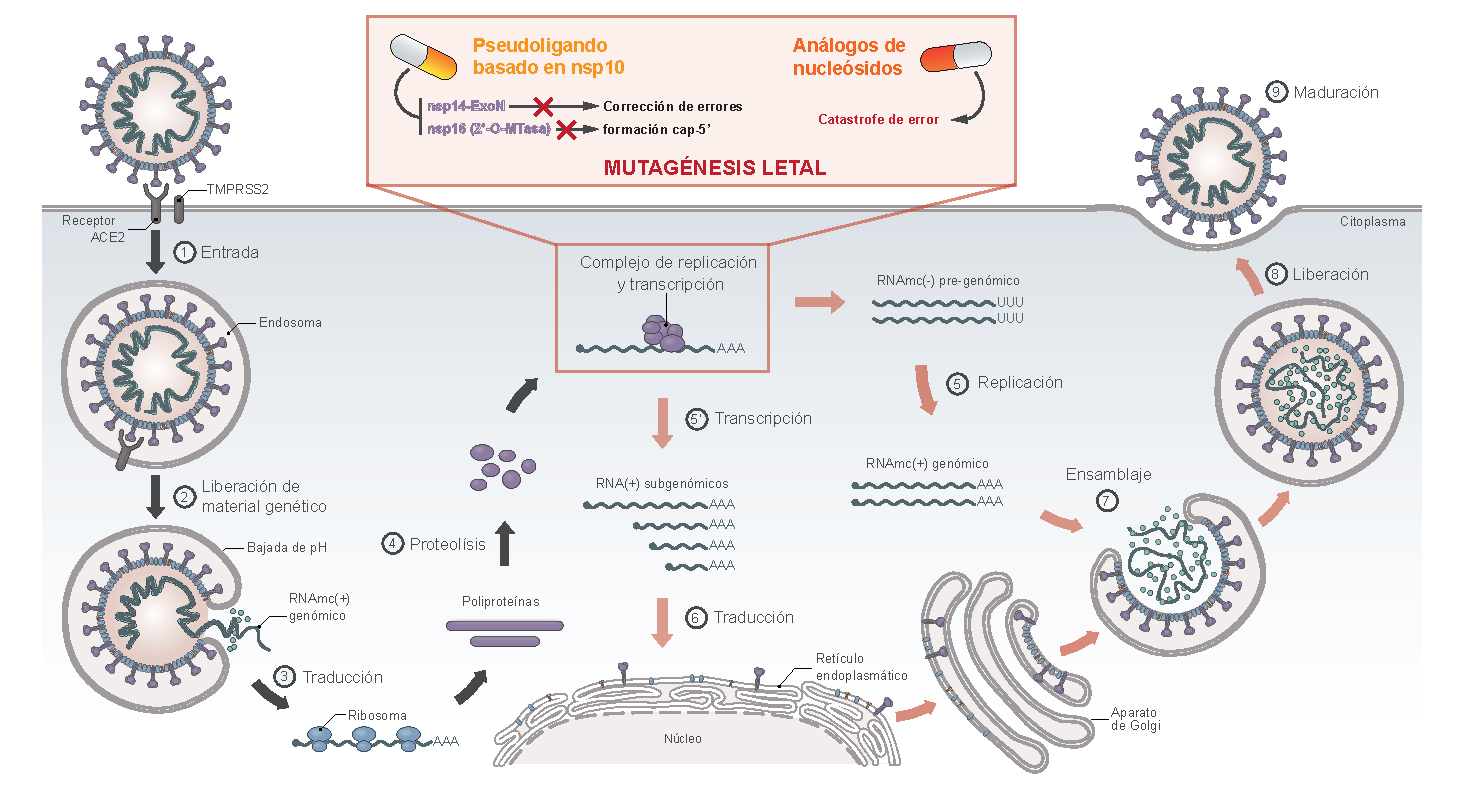
\includegraphics[width=1\textwidth]{img/fig3.pdf}
    \caption{Ciclo replicativo del SARS-CoV-2 y la estrategia antiviral 
    teórica que fundamenta los objetivos de este trabajo. La adición del 
    pseudoligando basado en nsp10 competiría por el sitio de interacción de 
    este mismo cofactor e impediría la correcta estabilización de las 
    actividades de nsp14-ExoN y nsp16. La supresión de estas enzimas 
    reduciría la fidelidad del complejo de replicación y transcripción (CRT)
    e inhibiría la formación del cap-5', exponiendo al genoma viral a su 
    degradación por la respuesta innata celular. Además, gracias a la 
    inactivación de la actividad correctora de la nsp14-ExoN, la adición de 
    análogos de bases aceleraría la tasa de mutación durante la replicación 
    y transcripción del genoma viral. Esto provocaría en el genoma del virus
    una pérdida acumulativa de su información (catástrofe de error), que 
    aceleraría la extinción del virus por acumulación de mutaciones letales 
    en su genoma. Figura adaptada de (\cite{asensio_ciclo_2020}).}\label{fig:cycle}
\end{sidewaysfigure}
